\section{Bilag}

\subsection{DCD}
\begin{figure}[H]
    \caption{Relation for vores DCD}
    \centering
        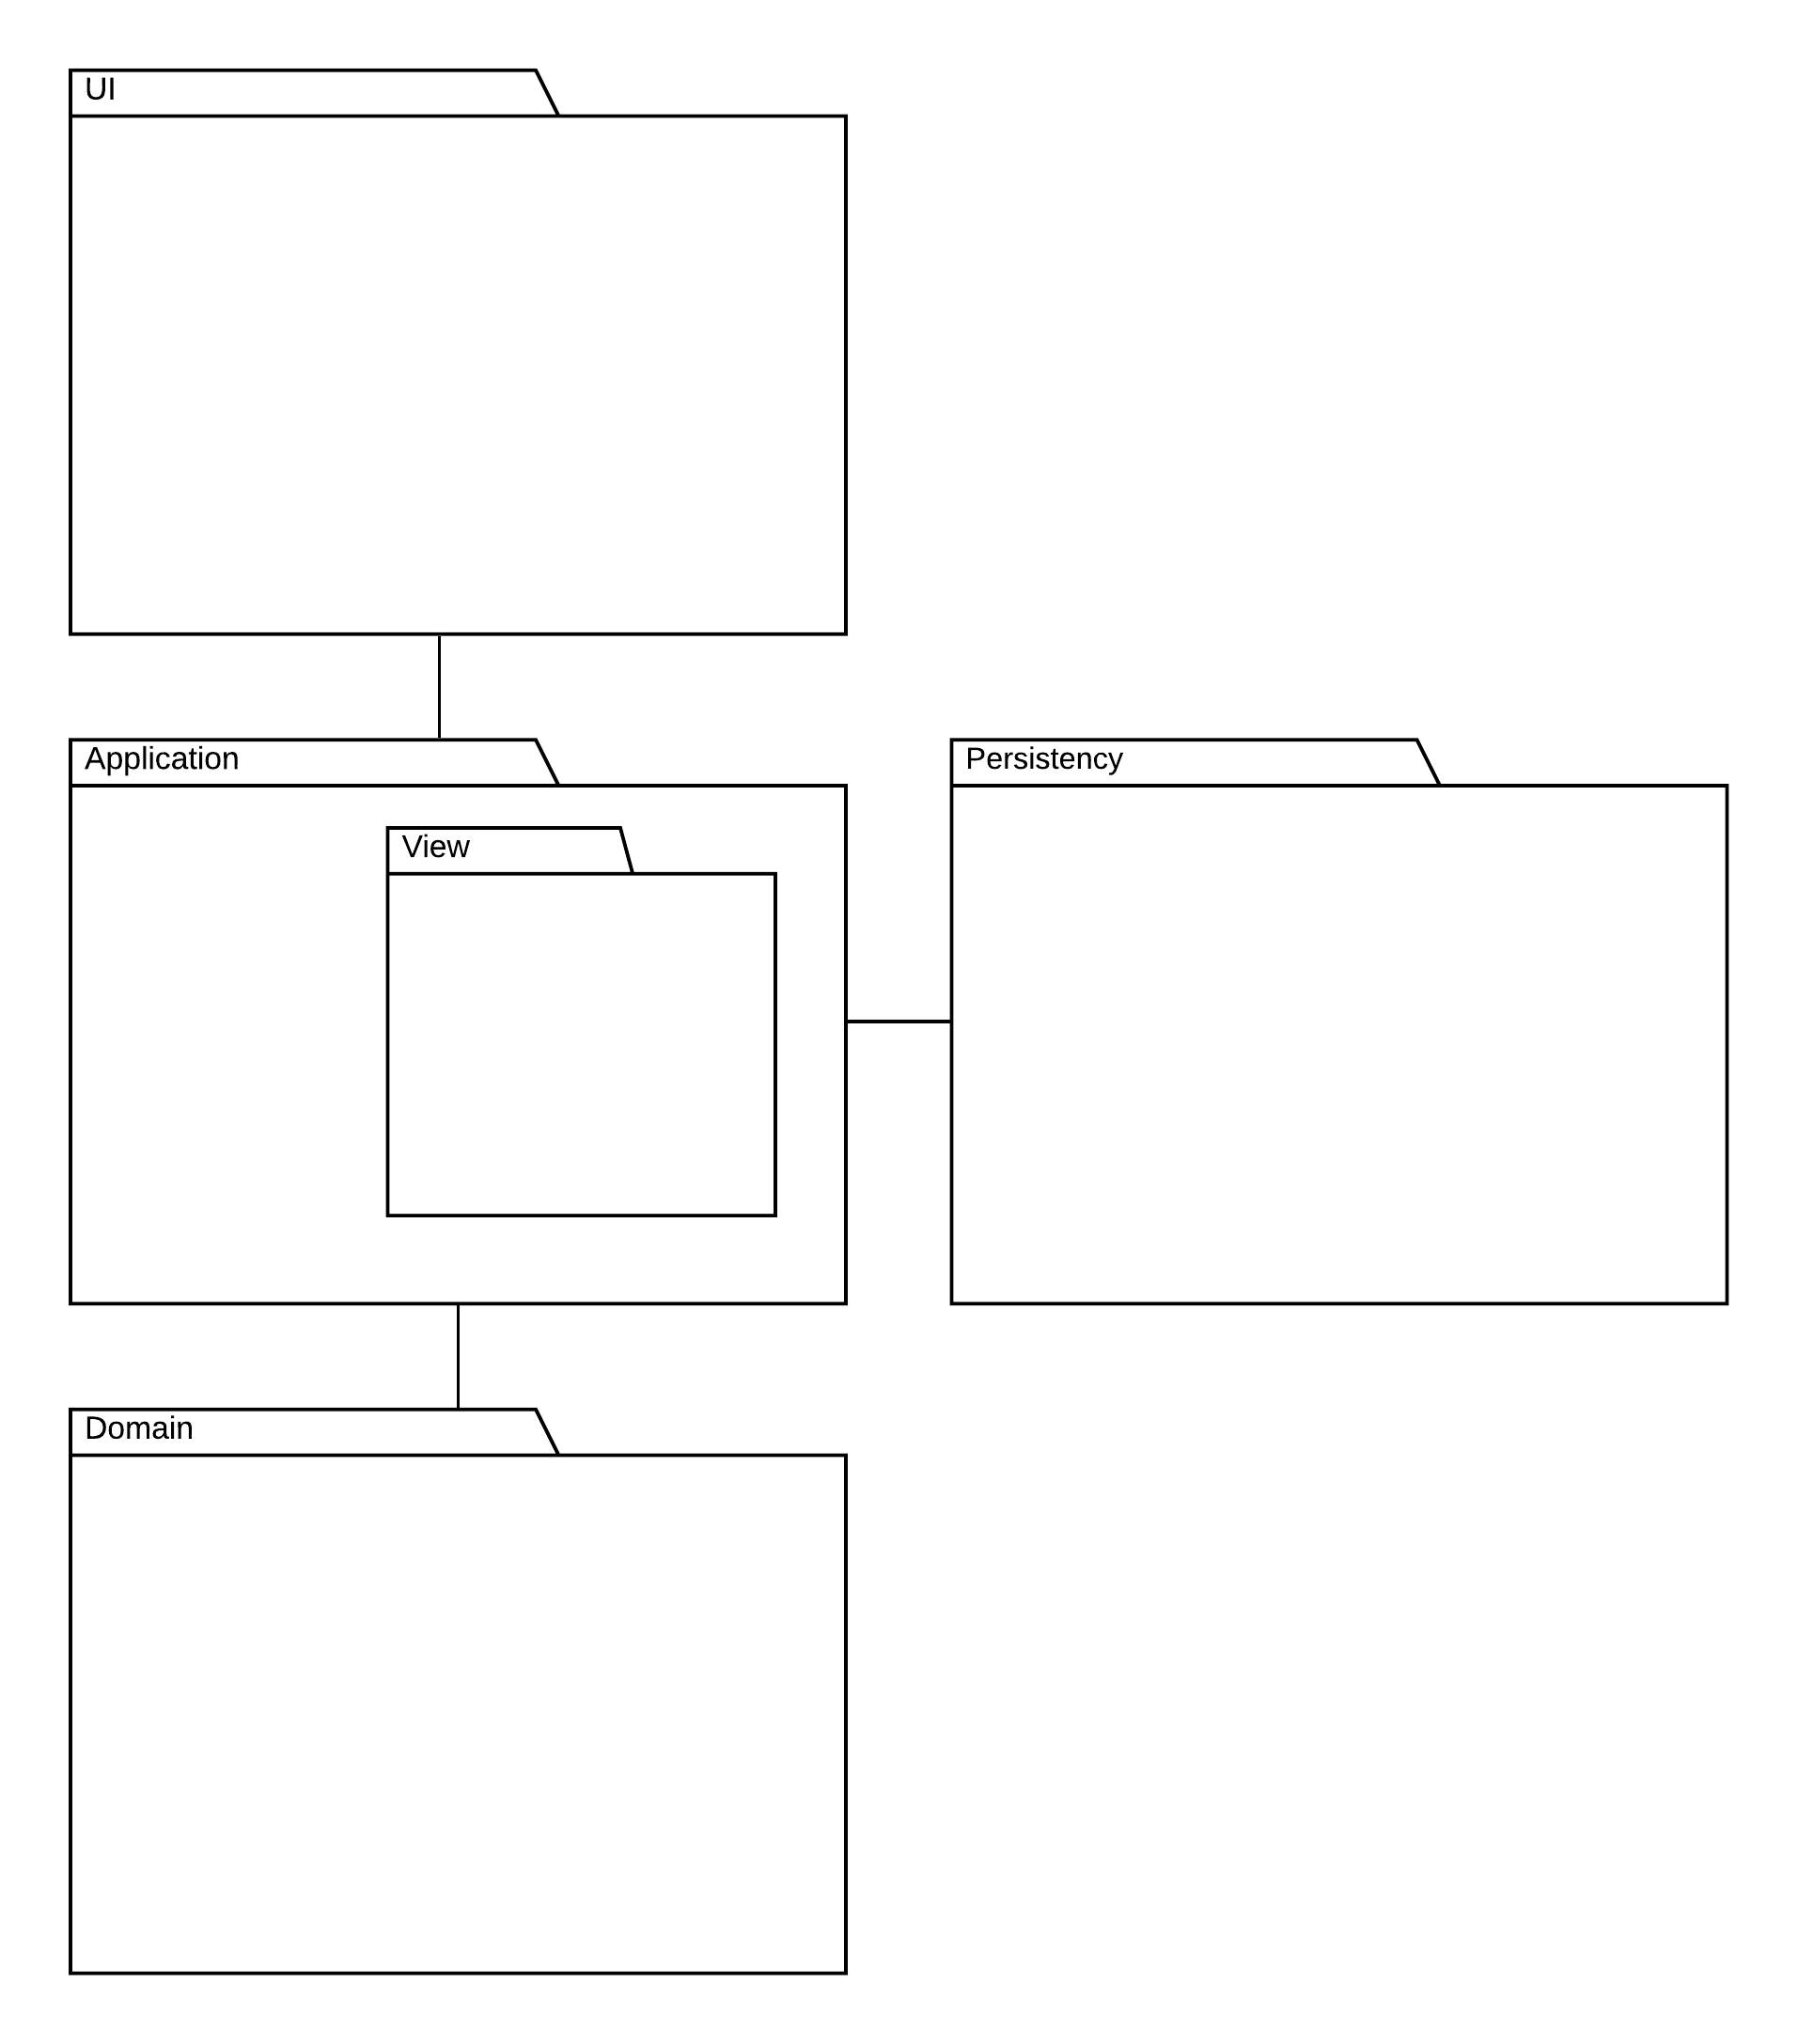
\includegraphics[width=\textwidth]{RelationDCD.png}
    \label{bilag:RelationDCD}
\end{figure}

\newpage
\begin{sidewaysfigure}[h]
    \caption{DCD for UI}
    \centering
        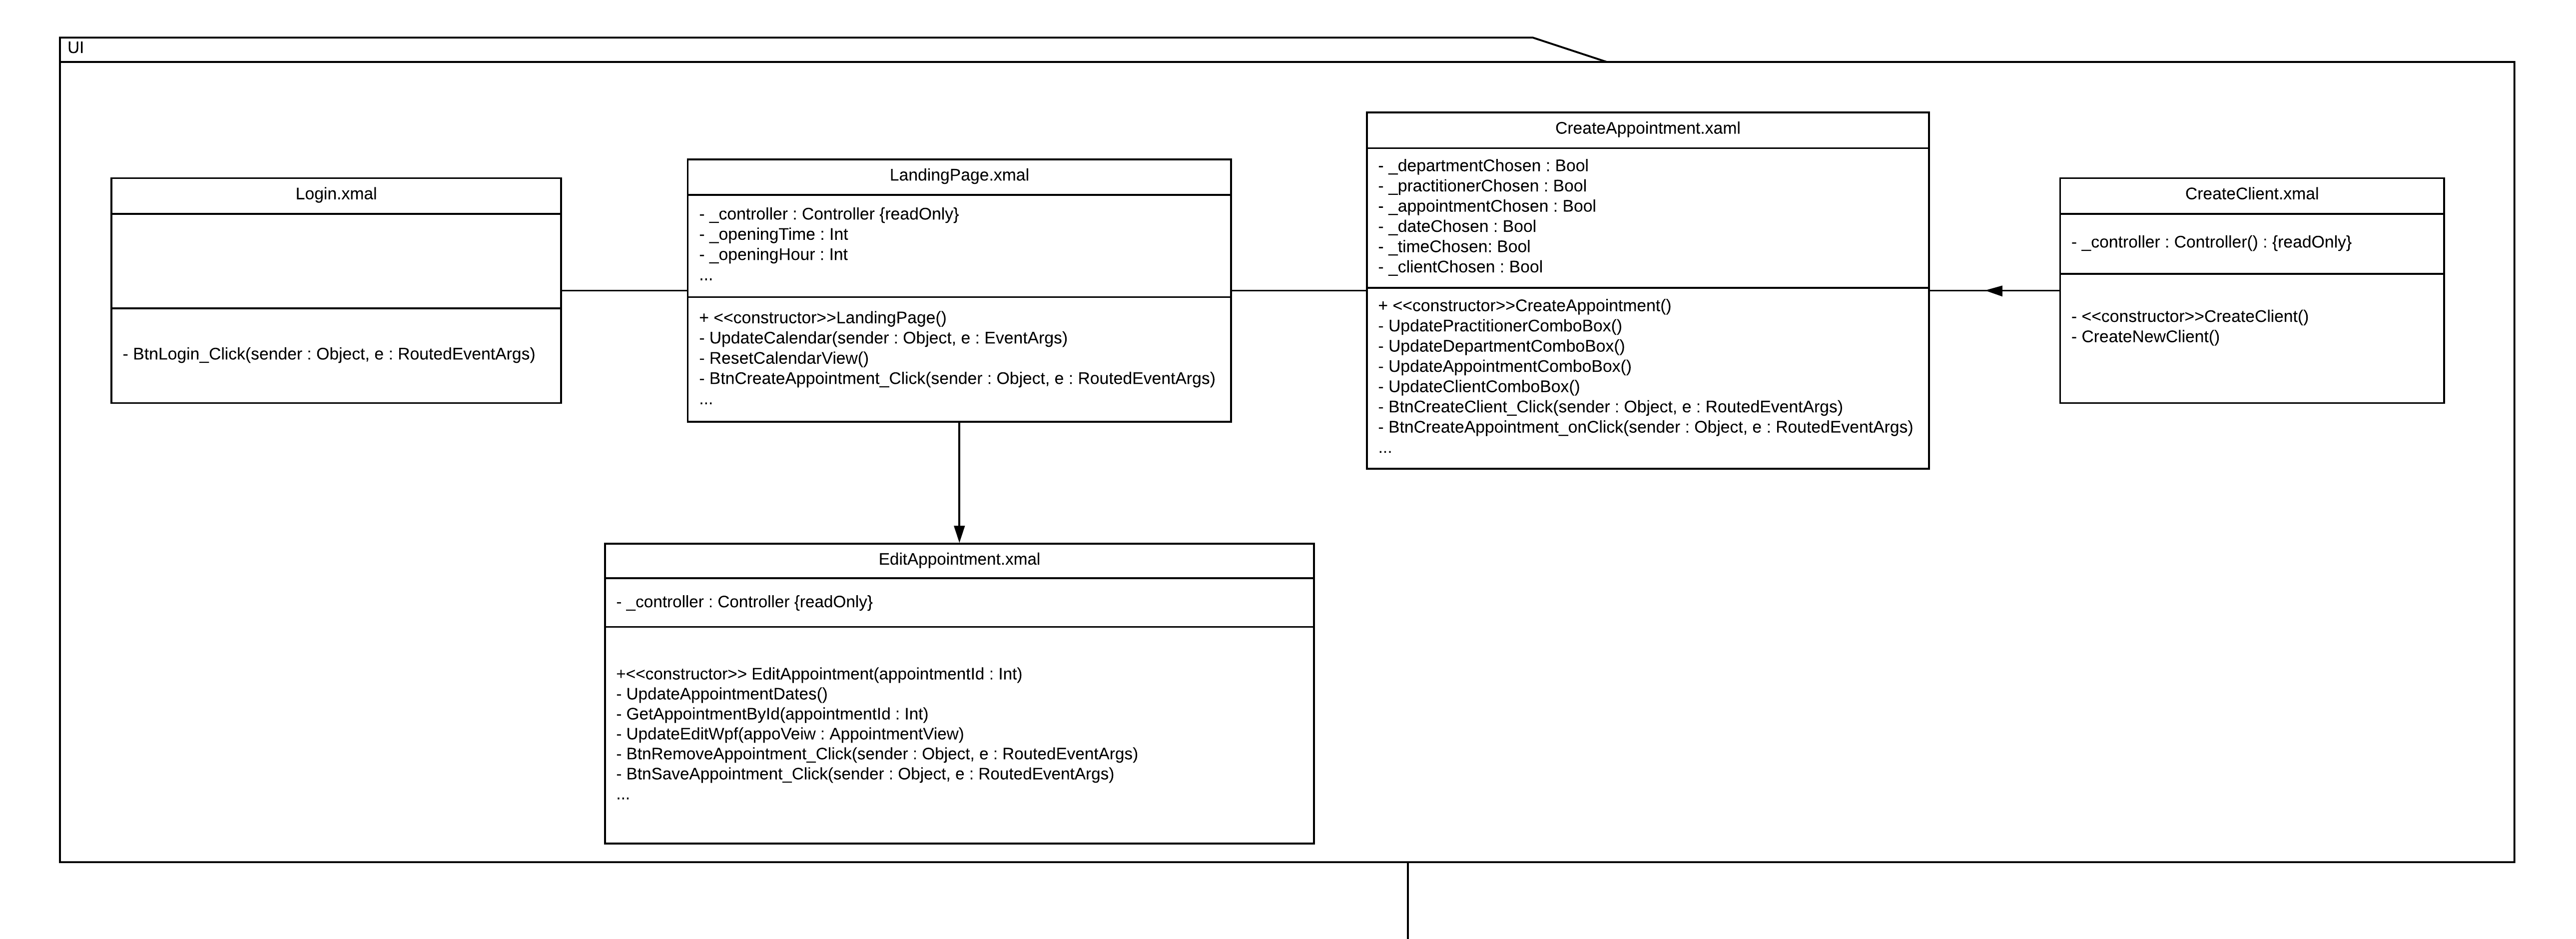
\includegraphics[width=\textwidth]{UIDCD.png}
    \label{bilag:UIDCD}
\end{sidewaysfigure}

\newpage
\begin{sidewaysfigure}[h]
    \caption{DCD for Application}
    \centering
        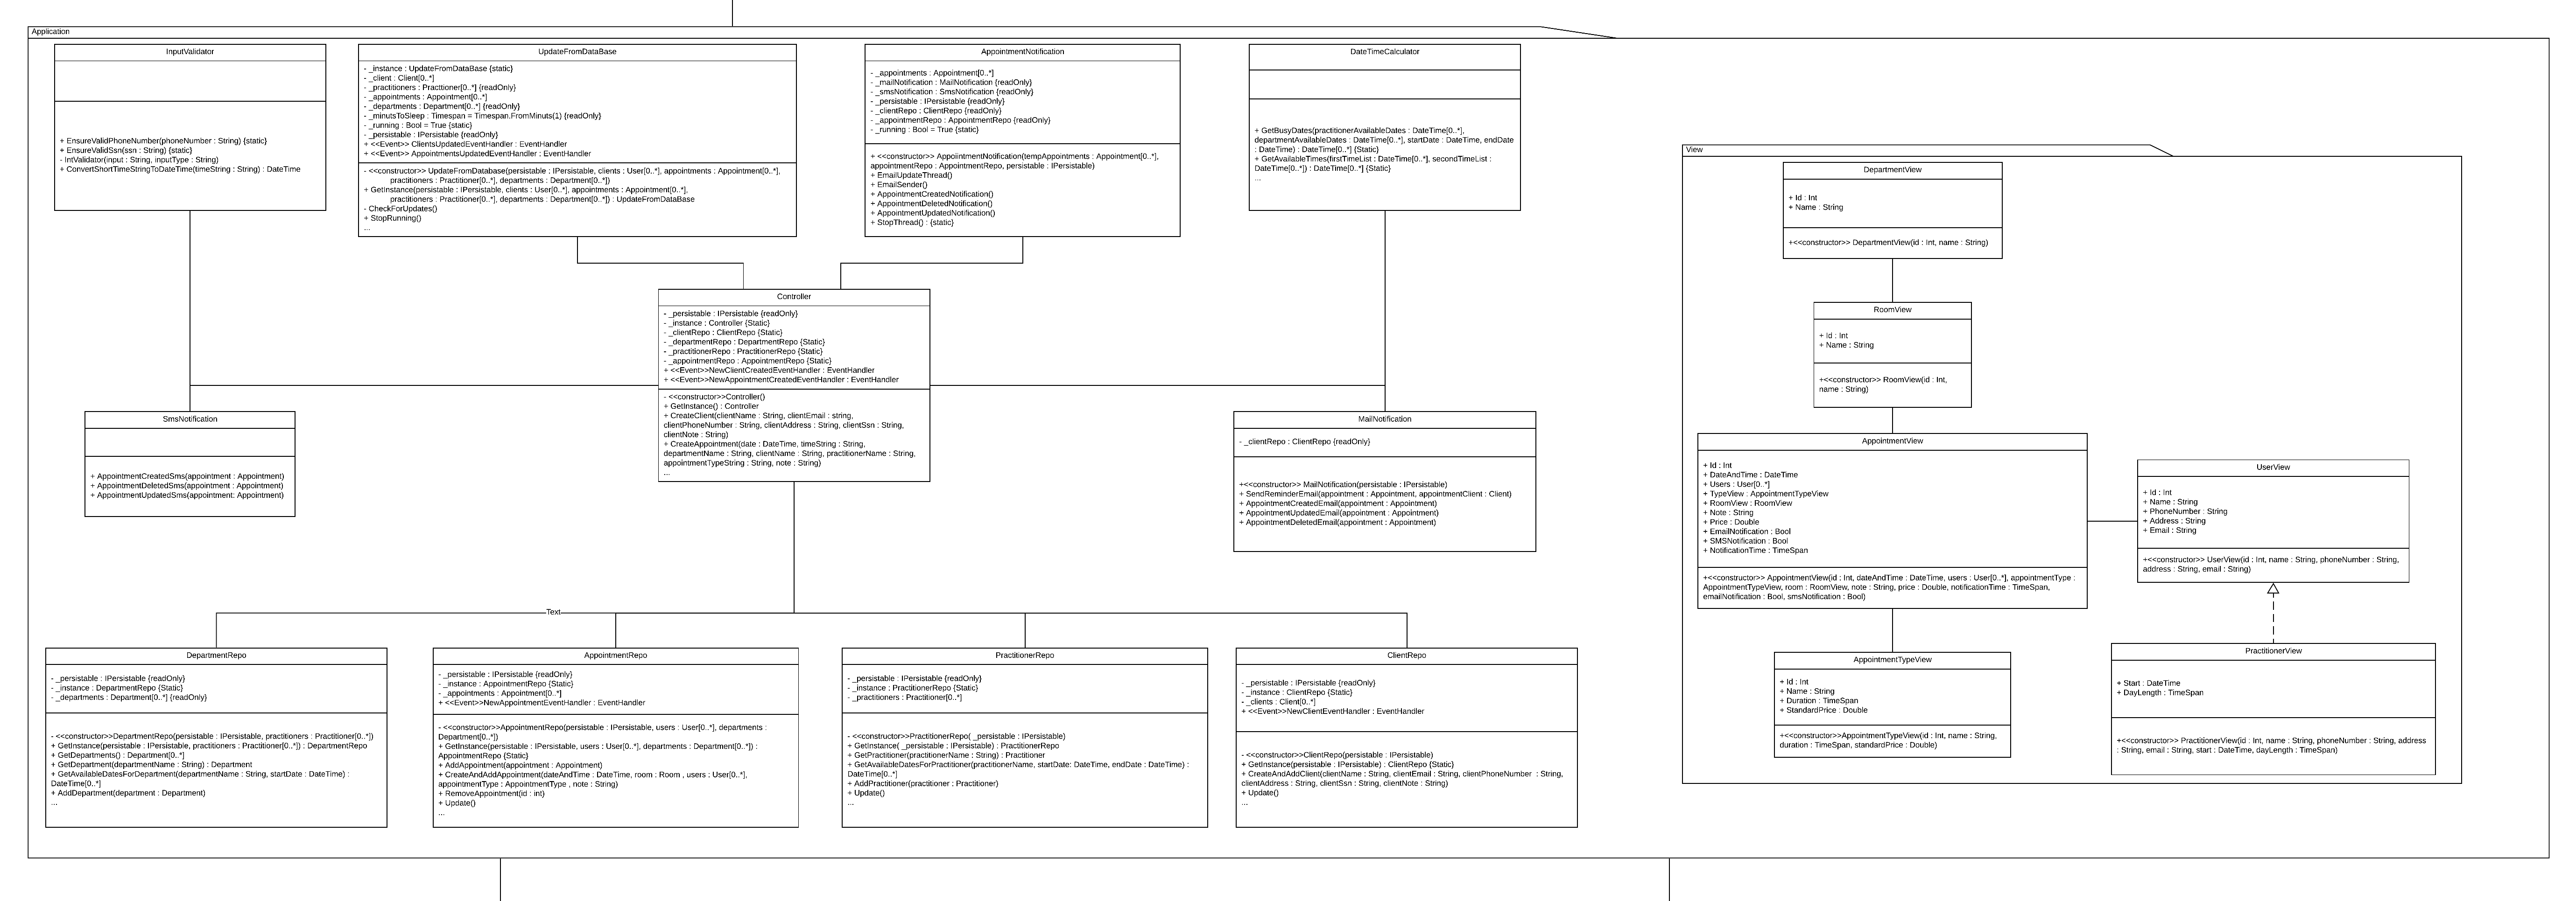
\includegraphics[width=\textwidth]{ApplicationDCD.png}
    \label{bilag:ApplicationDCD}
\end{sidewaysfigure}

\newpage
\begin{figure}[h]
    \caption{DCD for Domain}
    \centering
        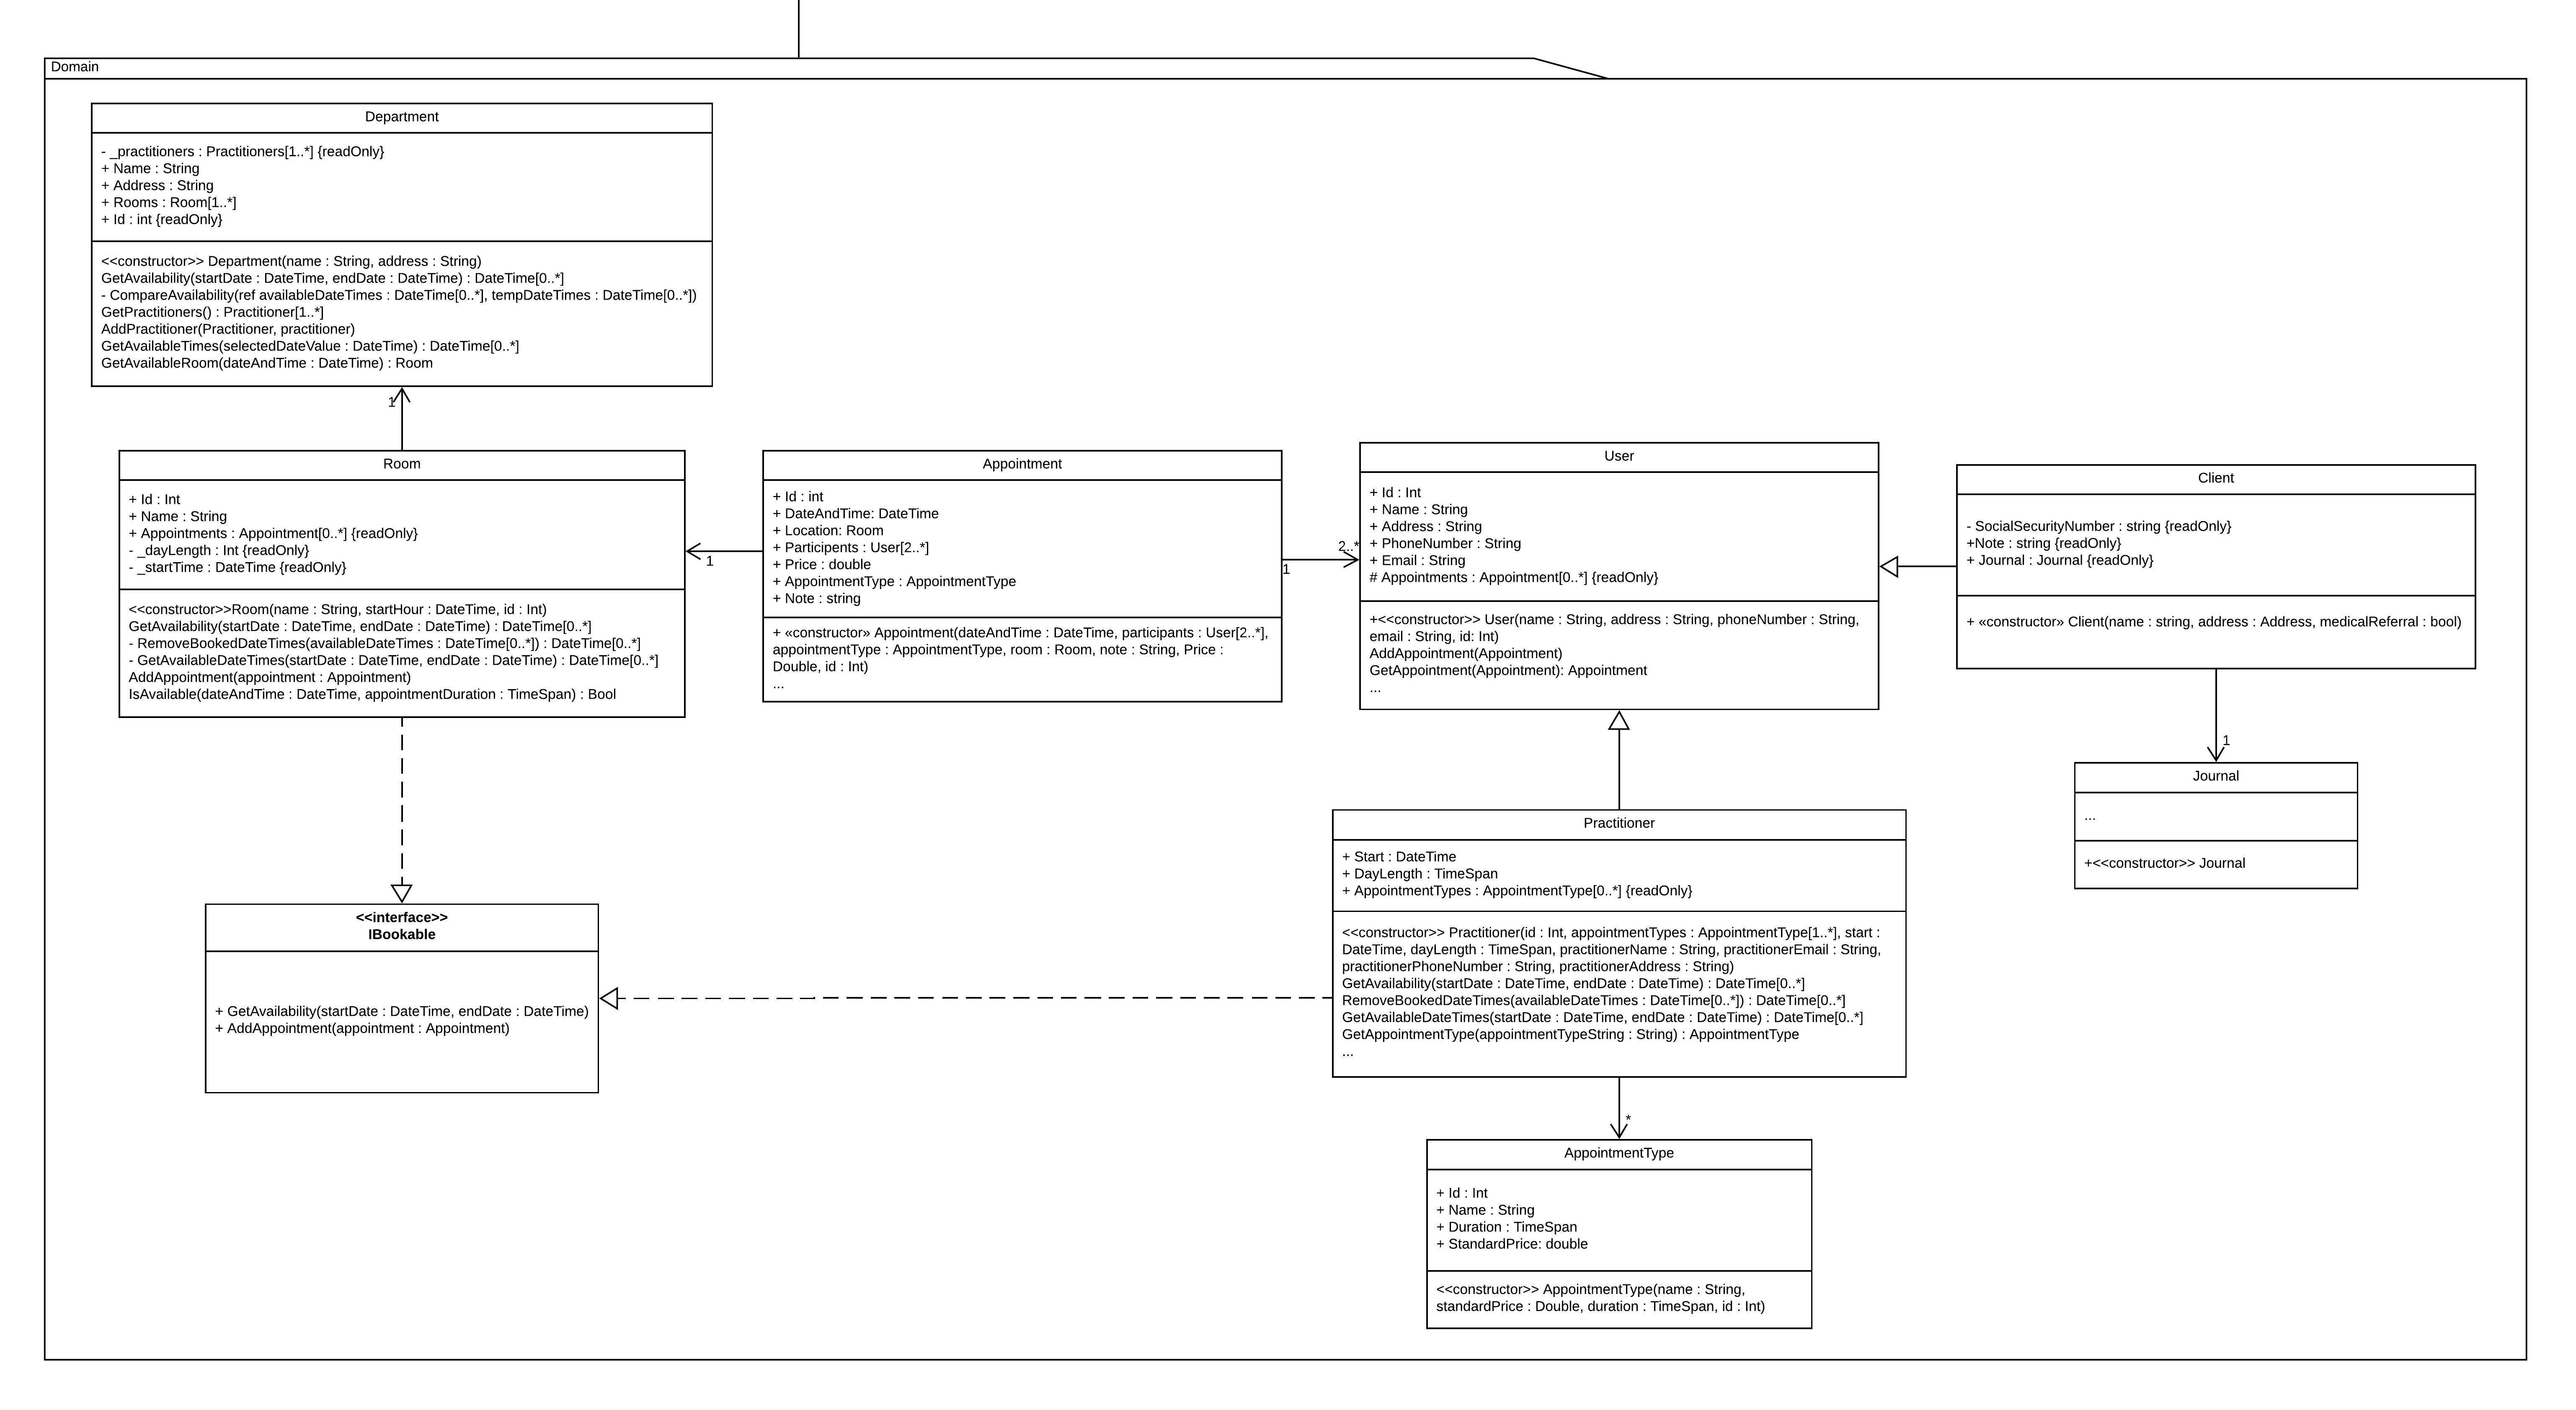
\includegraphics[width=\textwidth]{DomainDCD.png}
    \label{bilag:DomainDCD}
\end{figure}

\begin{figure}[h]
    \caption{DCD for Persistency}
    \centering
        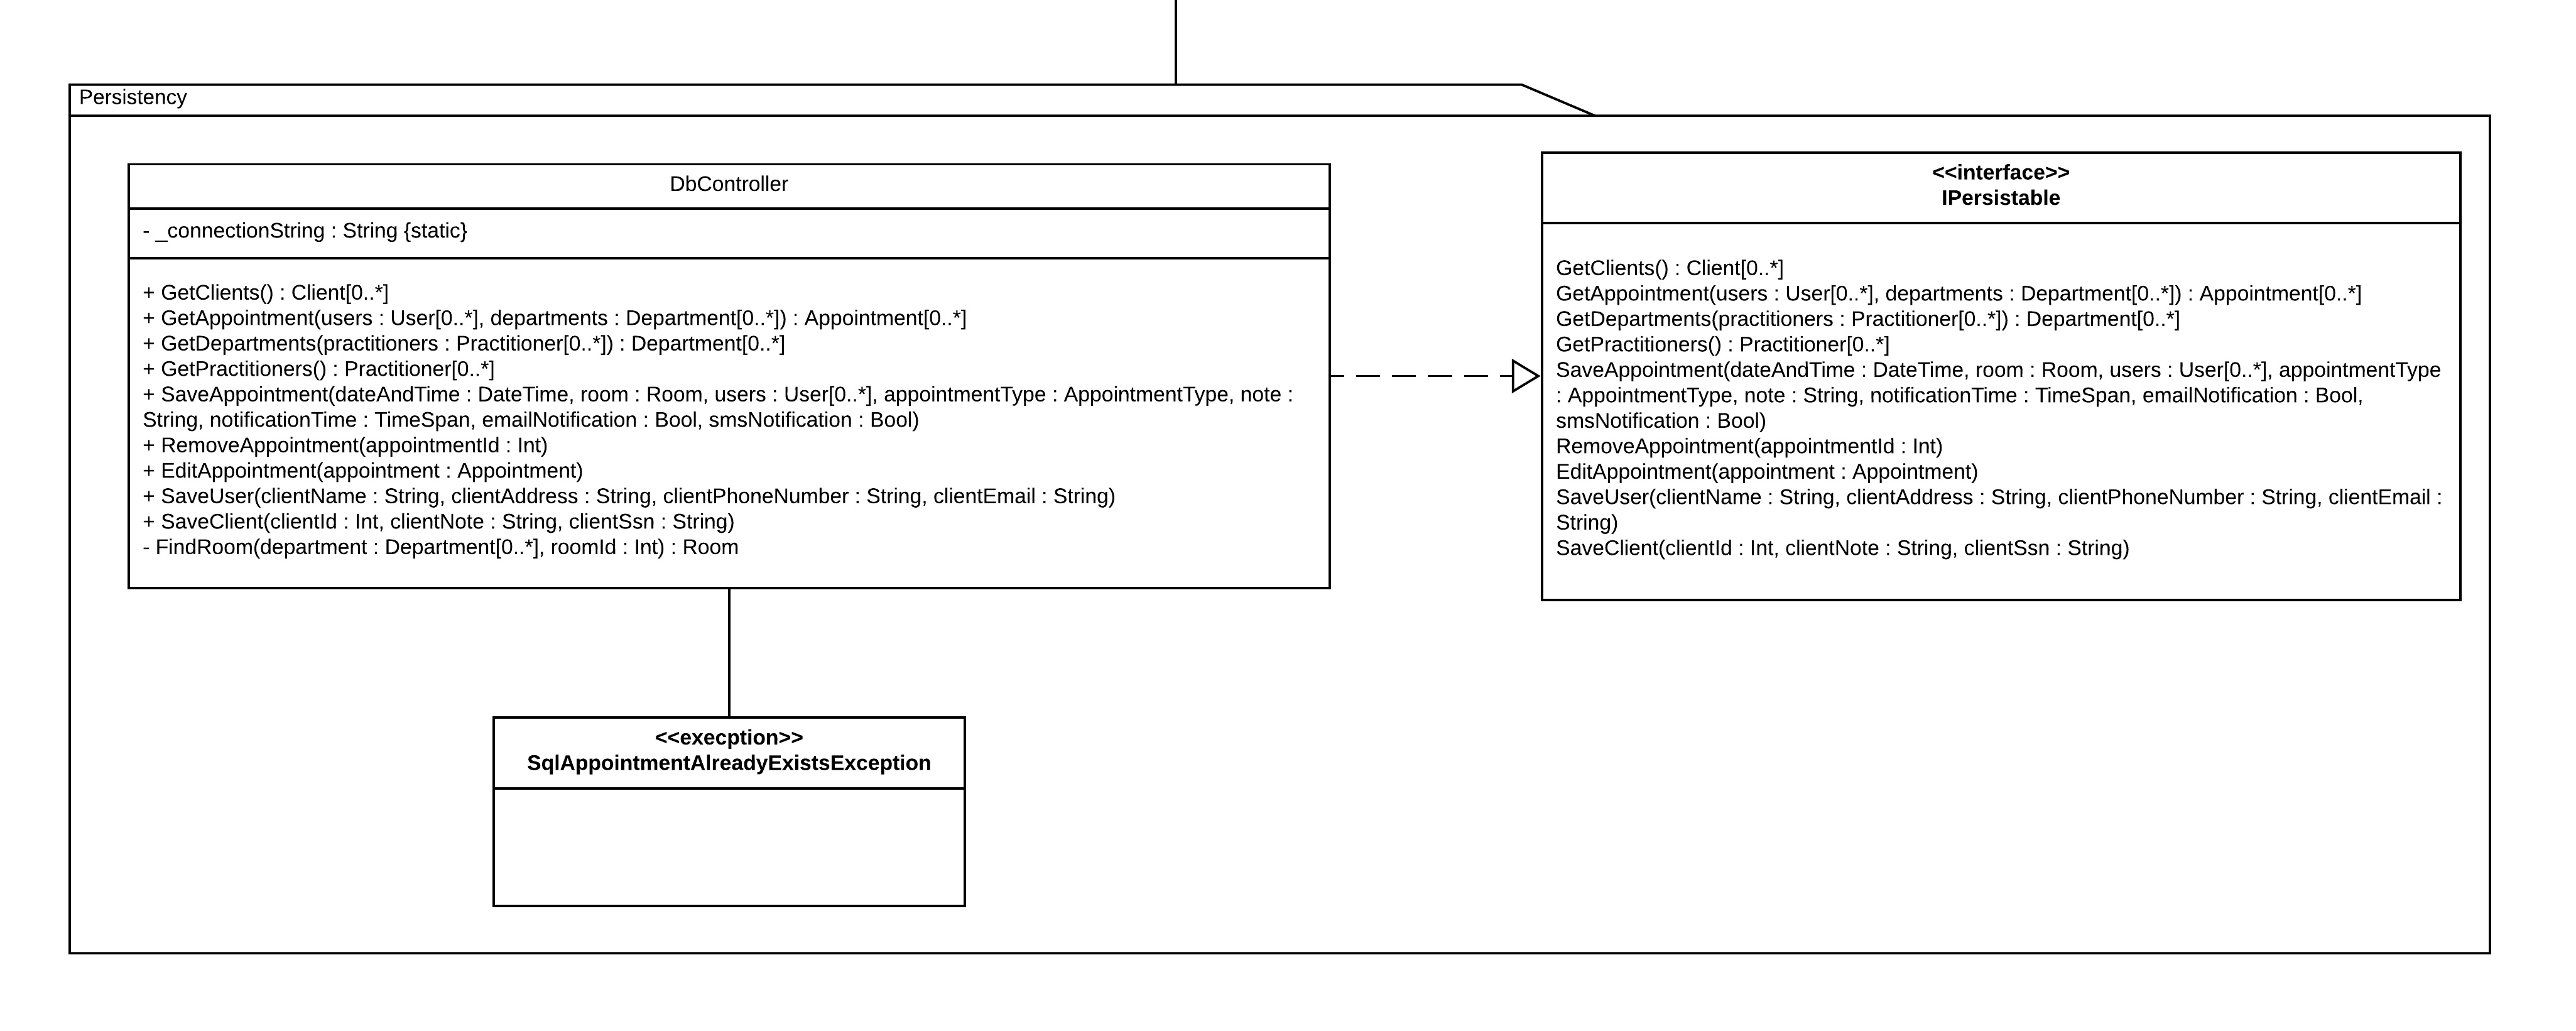
\includegraphics[width=\textwidth]{PersistableDCD.png}
    \label{bilag:PersistableDCD}
\end{figure}


\subsection{Kode}

\begin{figure}[h]
    \caption{Hjælpemetoder til CheckForUpdates metoden}
    \centering
        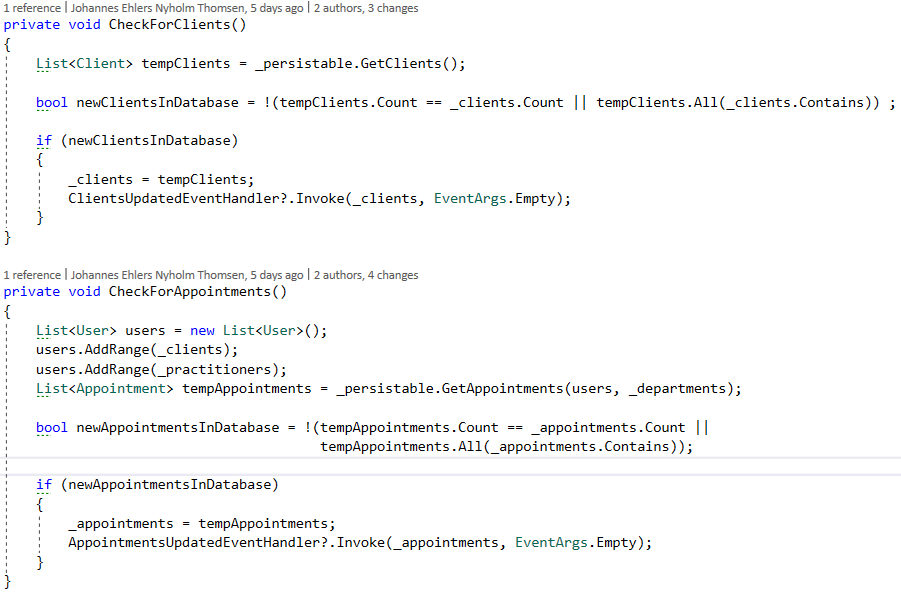
\includegraphics[width=\textwidth]{UpdateFromDatabaseHelpMethods.png}
    \label{bilag:CheckForUpdates }
\end{figure}

\subsection{ProjektLog}

% Please add the following required packages to your document preamble:
% \usepackage{graphicx}
% \usepackage[table,xcdraw]{xcolor}
% If you use beamer only pass "xcolor=table" option, i.e. \documentclass[xcolor=table]{beamer}
% \usepackage{lscape}
\begin{landscape}
\begin{table}[]
\centering
\resizebox{\linewidth}{!}{%
\begin{tabular}{|l|l|l|l|l|}
\hline
Dato & \textbf{I dag} & \multicolumn{3}{l|}{\textbf{Næste gang}} \\ \hline
\textbf{} & \textbf{Hvad har vi lavet indtil nu?} & \cellcolor[HTML]{D6D3CD}\textbf{Hvad er vi ikke blevet færdige med i dag?} & \textbf{Hvilke læringsmål skal vi arbejde (mere) med?} & \cellcolor[HTML]{D6D3CD}\textbf{Hvad skal vi arbejde med næste gang?} \\ \hline
\textbf{22/04/19} & \begin{tabular}[c]{@{}l@{}}Haft første møde \\ med Effektiv Landbrug\end{tabular} & \cellcolor[HTML]{D6D3CD} &  & \cellcolor[HTML]{D6D3CD} \\ \hline
\textbf{27/04/19} & \begin{tabular}[c]{@{}l@{}}Havde første møde \\ med Kommune Konsulterne/Psykolog Nord\end{tabular} & \cellcolor[HTML]{D6D3CD} &  & \cellcolor[HTML]{D6D3CD} \\ \hline
\textbf{01/04/19} & \begin{tabular}[c]{@{}l@{}}Påbegyndt objektmodel, domænemodel, \\ FML, Usecase diagram, wireframe\end{tabular} & \cellcolor[HTML]{D6D3CD}\begin{tabular}[c]{@{}l@{}}objekt, domænemodel, FML,\\ Usecase diagram, wireframe\end{tabular} & \begin{tabular}[c]{@{}l@{}}Kvalitetssikre OM, DM, \\ FML, Usecase Diagram\\ \\ Påbegynde:\\ Organisiationsdiagram,\\ Business Case\\ Informationssystemsanalyse\\ \\ Arbejde videre med wireframe\end{tabular} & \cellcolor[HTML]{D6D3CD}Arbejde i par. \\ \hline
\textbf{02/04/19} & \begin{tabular}[c]{@{}l@{}}Arbejdede på wireframe,\\ påbegyndt forretningsdelen i\\ businesscasen,\\ lavede skabelon\\ til KPI'er. lavede organsationsdiagram\end{tabular} & \cellcolor[HTML]{D6D3CD}Businesscase, og KPI & \begin{tabular}[c]{@{}l@{}}Forsætte KPI'er \\ og påbegynde udretning af Usecases\end{tabular} & \cellcolor[HTML]{D6D3CD}Arbejde i par. \\ \hline
\textbf{03/04/19} & \begin{tabular}[c]{@{}l@{}}Lavede KPI'er, lavede use cases, forsat på business case, \\ påbegyndt interessentanalyse. Lavede Kodestandard.\end{tabular} & \cellcolor[HTML]{D6D3CD}Businesscase & Businesscase, navigationsdiagram. & \cellcolor[HTML]{D6D3CD}Arbejde i par, evt. selvstændigt. \\ \hline
\textbf{04/04/19} & \begin{tabular}[c]{@{}l@{}}Færdiggjorde interessentanalyse , \\ lavede analyse af valgte løsning. \\ Opstillede løsningsscenarier, \\ Lavede SSD'er, skrev KPI'er ind i rapporten, \\ lavede videre på use cases.\end{tabular} & \cellcolor[HTML]{D6D3CD}De sidste use cases. & \begin{tabular}[c]{@{}l@{}}Use Cases, SOC'er. \\ Problemmodellering/Artefakter i rapporten. \\ Liste over kapitler i rapport. \\ Vidensdeling med anden gruppe.\end{tabular} & \cellcolor[HTML]{D6D3CD}Arbejde i par, evt. selvstændigt. \\ \hline
\textbf{05/04/19} & \begin{tabular}[c]{@{}l@{}}Lavede vidensdeling med anden gruppe. \\ Liste over kapitler i rapport.\\ \\ Møde med vejledere\end{tabular} & \cellcolor[HTML]{D6D3CD}Testing af SSD'er, SOC'er, Use Cases. & \begin{tabular}[c]{@{}l@{}}Rsikovurdering, Kvalitetsplan, \\ Rette Use Cases, \\ Rette SSD.\end{tabular} & \cellcolor[HTML]{D6D3CD}Arbejde i par, evt. selvstændigt. \\ \hline
\textbf{08/04/19} & \begin{tabular}[c]{@{}l@{}}Færdiggjorde SSD'er. Lavede risikoanalyse , \\ lavede udkast af navigationsdiagram. Påbegyndt SOC.\end{tabular} & \cellcolor[HTML]{D6D3CD} & \begin{tabular}[c]{@{}l@{}}Definition of done, kvalitetsplan, \\ Rette Use Cases.\end{tabular} & \cellcolor[HTML]{D6D3CD}\begin{tabular}[c]{@{}l@{}}Arbejde selvstændigt, evt. Par.\\ \\ Find evt. Et rum (no reddit bitches)\end{tabular} \\ \hline
\textbf{09/04/19} & \begin{tabular}[c]{@{}l@{}}Lavede kvalitetsplan, definition of done, \\ kiggede på læringsmål \\ og deres relation til rapportens indhold. \\ Lavede videre på SOC.\end{tabular} & \cellcolor[HTML]{D6D3CD}SOC'er, rette use cases, arkitekttur af løsningen. & \begin{tabular}[c]{@{}l@{}}Arkitetur af løsningen, SOC'er, \\ Rette Use Cases.\end{tabular} & \cellcolor[HTML]{D6D3CD}\begin{tabular}[c]{@{}l@{}}Arbejde selvstændigt, evt. Par.\\ \\ Find evt. Et rum (no reddit bitches)\end{tabular} \\ \hline
\textbf{10/04/19} & \begin{tabular}[c]{@{}l@{}}Lavede videre på Wireframe, Holdte møde med vejledere.\\ Reviewede Kvalitetsplan.\end{tabular} & \cellcolor[HTML]{D6D3CD}Arkitetur af læsningen, SOC'er, rette use cases. & \begin{tabular}[c]{@{}l@{}}Gå igennem review tasks.\\ \\ Feedback fra vejledere.\\ \\ Arkitektur af løsningen, SOC'er, \\ rette use cases.\end{tabular} & \cellcolor[HTML]{D6D3CD}\begin{tabular}[c]{@{}l@{}}Arbejde selvstændigt, evt. Par.\\ \\ Find evt. Et rum.\end{tabular} \\ \hline
\textbf{11/04/19} & \begin{tabular}[c]{@{}l@{}}Rettede ud fra vejleder feedback, \\ læst korrektur, reviewede løsningsscenarier. \\ \\ Vidensdeling på tværs af klassen af vurderingskriterier. \\ \\ Snakkede om Hans om navigations. diagra \\ og læringsmålene\end{tabular} & \cellcolor[HTML]{D6D3CD}\begin{tabular}[c]{@{}l@{}}Feedback fra vejleder (KPI). \\ \\ Arkitektur af løsningen, SOC’er, rette use cases.\end{tabular} & \begin{tabular}[c]{@{}l@{}}Forsæt med review tasks.  \\ \\ Vidensdeling med anden gruppe\\ (Use Cases).  \\ \\ Møde med PO.  \\ \\ Feedback fra vejleder (KPI)\end{tabular} & \cellcolor[HTML]{D6D3CD}\begin{tabular}[c]{@{}l@{}}Arbejde selvstændigt, evt. Par. \\ \\ Find evt. Et rum. \\ \\ Møde med PO ved A4.34\end{tabular} \\ \hline
\textbf{12/04/19} & \begin{tabular}[c]{@{}l@{}}Sparing med anden gruppe (Use Cases). \\ \\ Sprint retrospektiv. \\  \\ Forsatte med review tasks. \\  \\ Holdte møde med PO.\end{tabular} & \cellcolor[HTML]{D6D3CD}\begin{tabular}[c]{@{}l@{}}Forsæt med review tasks, mangler use cases.\\ \\ Feedback fra vejleder (KPI)\end{tabular} & \begin{tabular}[c]{@{}l@{}}Påbegynd Sprint 1.\\ \\ Hold SCRUM meeting.\\ \\ Kør planning poker.\\ \\ Rette use cases, påskeferien.\end{tabular} & \cellcolor[HTML]{D6D3CD}\begin{tabular}[c]{@{}l@{}}Arbejde selvstændigt, evt. et par.\\ \\ Find evt. et rum.\end{tabular} \\ \hline
\end{tabular}%
}
\end{table}
\end{landscape}

% Please add the following required packages to your document preamble:
% \usepackage{graphicx}
% \usepackage[table,xcdraw]{xcolor}
% If you use beamer only pass "xcolor=table" option, i.e. \documentclass[xcolor=table]{beamer}
% \usepackage{lscape}
\begin{landscape}
\begin{table}[]
\centering
\resizebox{\linewidth}{!}{%
\begin{tabular}{|l|l|l|l|l|}
\hline
Dato & \textbf{I dag} & \multicolumn{3}{l|}{\textbf{Næste gang}} \\ \hline
\textbf{} & \textbf{Hvad har vi lavet indtil nu?} & \cellcolor[HTML]{D6D3CD}\textbf{Hvad er vi ikke blevet færdige med i dag?} & \textbf{Hvilke læringsmål skal vi arbejde (mere) med?} & \cellcolor[HTML]{D6D3CD}\textbf{Hvad skal vi arbejde med næste gang?} \\ \hline
\textbf{23/04/19} & \begin{tabular}[c]{@{}l@{}}Holdt planning poker og SCRUM meeting for sprint 1.\\ \\ Rettede use cases og SSD'er.\\ \\ Påbegyndt på UI, DCD, DBD og SOC'er.\end{tabular} & \cellcolor[HTML]{D6D3CD}UI, DCD, DBD og SOC'er & \begin{tabular}[c]{@{}l@{}}Forsæt på UI, DCD, DBD og SOC'er.\\ \\ Påbegyndt SD'er.\end{tabular} & \cellcolor[HTML]{D6D3CD}\begin{tabular}[c]{@{}l@{}}Arbejde selvstændigt, evt. par.\\ \\ Find evt. Et rum.\end{tabular} \\ \hline
\textbf{24/04/19} & \begin{tabular}[c]{@{}l@{}}Lavede videre på SOC'er, UI, DBD, DCD.\\ \\ Påbegyndt på BPMN for efter system, SD'er, implementering af metoderne.\\ \\ Rettede SOC'er.\end{tabular} & \cellcolor[HTML]{D6D3CD}UI, DCD, DBD, SD'er, implementering. & \begin{tabular}[c]{@{}l@{}}Forsæt på UI, DBD, DCD, SD'er \\ og implementering af kode.\\ \\ Kvalitetssikre BPMN.\end{tabular} & \cellcolor[HTML]{D6D3CD}\begin{tabular}[c]{@{}l@{}}Arbejde selvstændigt, evt. par.\\ \\ Find evt. Et rum.\end{tabular} \\ \hline
\textbf{25/04/19} & \begin{tabular}[c]{@{}l@{}}Lavede UI landing page færdig. \\ \\ Forsat på implementering af book ny aftale.\\ \\ Påbegyndt af opsætning af database.\end{tabular} & \cellcolor[HTML]{D6D3CD}\begin{tabular}[c]{@{}l@{}}DCD, DBD, SD'er, implementering af kode.\\ \\ Kvalitetssikre BPMN.\end{tabular} & \begin{tabular}[c]{@{}l@{}}Forsæt på DBD, DCD, SD'er \\ og implementering af kode.\\ \\ Kvalitetssikre BPMN.\end{tabular} & \cellcolor[HTML]{D6D3CD}\begin{tabular}[c]{@{}l@{}}Arbejde selvstændigt, evt. par.\\ \\ Find evt. Et rum.\end{tabular} \\ \hline
\textbf{26/04/19} & \begin{tabular}[c]{@{}l@{}}Forsat implementering.\\ \\ Lavede rapport over SSD'er og SOC'er.\\ \\ Kvalitetssikrede BPMN.\\ \\ Reviewede SSD'er, DBD.\\ \\ DBD tilbage i "To Do"\end{tabular} & \cellcolor[HTML]{D6D3CD}DCD, DBD, SD'er, implementering af kode. & \begin{tabular}[c]{@{}l@{}}Forsæt på DBD, DCD, SD'er \\ og implementering af kode.\end{tabular} & \cellcolor[HTML]{D6D3CD}\begin{tabular}[c]{@{}l@{}}Arbejde selvstændigt, evt. par.\\ \\ Find evt. et rum.\end{tabular} \\ \hline
\textbf{29/04/19} & \begin{tabular}[c]{@{}l@{}}Forsat implementering af use case.\\ \\ Reviewede BPMN, SD'er.\\ \\ Påbegyndt rettelse af DCD.\\ \\ Rettede rapport efter feedback fra PO.\\ \\ Skrevet på SOC'er og SSD'er kapitler.\end{tabular} & \cellcolor[HTML]{D6D3CD}Ikke rigtigt noget, det kører. & \begin{tabular}[c]{@{}l@{}}Forsæt på DBD, DCD \\ og implementering af kode.\end{tabular} & \cellcolor[HTML]{D6D3CD}\begin{tabular}[c]{@{}l@{}}Arbejde selvstændigt, evt. Par.\\ \\ Find evt. Et rum.\end{tabular} \\ \hline
\textbf{30/04/19} & \begin{tabular}[c]{@{}l@{}}Fortsat implementering af kode.\\ \\ Lavede Stored Procedures til DB.\\ \\ Rettede DC, lavede SD'er og SOC'er for faktura.\\ \\ Reviewede rapportrettelser og SP'er.\end{tabular} & \cellcolor[HTML]{D6D3CD}\begin{tabular}[c]{@{}l@{}}Ikke rigtigt noget.\\ Det kører.\end{tabular} & \begin{tabular}[c]{@{}l@{}}Forsæt implementering af kode. Lave SD'er og SOC'er.\\ \\ Evt. Rapportskrivning\end{tabular} & \cellcolor[HTML]{D6D3CD}\begin{tabular}[c]{@{}l@{}}Arbejde selvstændigt, evt. Par.\\ \\ Find evt. Et rum.\end{tabular} \\ \hline
\textbf{01/05/19} & \begin{tabular}[c]{@{}l@{}}Forsat implementering af kode.\\ \\ Færdiggjorde Stored Procedures til DB.\\ \\ Lavede UI.\\ \\ Påbegyndt implementering af DB-controller.\end{tabular} & \cellcolor[HTML]{D6D3CD}Review-sager & \begin{tabular}[c]{@{}l@{}}Forsat implementering af kode og DB-controlle.\\ \\ Fortsæt arbejde på UI.\\ \\ Review ting i review.\end{tabular} & \cellcolor[HTML]{D6D3CD}\begin{tabular}[c]{@{}l@{}}Arbejde selvstændigt, evt. Par.\\ \\ Find evt. Et rum.\end{tabular} \\ \hline
\textbf{02/05/19} & \begin{tabular}[c]{@{}l@{}}Forsat implementering af kode.\\ \\ Ændrede på Database.\\ \\ Færdiggjort UI.\\ \\ Reviewede SOC'er og SSD'er for Se faktura.\end{tabular} & \cellcolor[HTML]{D6D3CD} & \begin{tabular}[c]{@{}l@{}}Fortsæt implementering af kode og DB-controller.\\ \\ Review ting i review.\end{tabular} & \cellcolor[HTML]{D6D3CD}\begin{tabular}[c]{@{}l@{}}Arbejde selvstændigt, evt. Par.\\ \\ Find evt. Et rum.\end{tabular} \\ \hline
\textbf{03/05/19} & \begin{tabular}[c]{@{}l@{}}Lavede sprint reivew, lavede happines index.\\ \\ Forsat implementering af kode.\\ \\ Ændrede på Database.\end{tabular} & \cellcolor[HTML]{D6D3CD} & \begin{tabular}[c]{@{}l@{}}Fortsæt implementering af kode og DB-controller.\\ \\ Review ting i review.\end{tabular} & \cellcolor[HTML]{D6D3CD}\begin{tabular}[c]{@{}l@{}}Arbejde selvstændigt, evt. Par.\\ \\ Find evt. Et rum.\end{tabular} \\ \hline
\end{tabular}%
}
\end{table}
\end{landscape}


% Please add the following required packages to your document preamble:
% \usepackage{graphicx}
% \usepackage[table,xcdraw]{xcolor}
% If you use beamer only pass "xcolor=table" option, i.e. \documentclass[xcolor=table]{beamer}
% \usepackage{lscape}
\begin{landscape}
\begin{table}[]
\centering
\resizebox{\linewidth}{!}{%
\begin{tabular}{|l|l|l|l|l|}
\hline
Dato & \textbf{I dag} & \multicolumn{3}{l|}{\textbf{Næste gang}} \\ \hline
\textbf{} & \textbf{Hvad har vi lavet indtil nu?} & \cellcolor[HTML]{D6D3CD}\textbf{Hvad er vi ikke blevet færdige med i dag?} & \textbf{Hvilke læringsmål skal vi arbejde (mere) med?} & \cellcolor[HTML]{D6D3CD}\textbf{Hvad skal vi arbejde med næste gang?} \\ \hline
\textbf{06/05/19} & \begin{tabular}[c]{@{}l@{}}Lavede DB, SP, DB-controller.\\ Lavede Rapportskrivning.\\ Lavede Pakkediagram.\end{tabular} & \cellcolor[HTML]{D6D3CD}DB, SP, DB-controller, Planning Poker & Planning Poker, Se Faktura artefakter. & \cellcolor[HTML]{D6D3CD}\begin{tabular}[c]{@{}l@{}}Arbejde selvstændigt, evt. Par.\\ \\ Find evt. Et rum.\end{tabular} \\ \hline
\textbf{07/05/19} & \begin{tabular}[c]{@{}l@{}}Lavede DB-controller\\ Skrev rapport.\\ Påbegyndte implementering af aflys aftale\end{tabular} & \cellcolor[HTML]{D6D3CD}Review sager & Oprette ny sprint ting, burndownchart. & \cellcolor[HTML]{D6D3CD}\begin{tabular}[c]{@{}l@{}}Arbejde selvstændigt, evt. Par.\\ \\ Find evt. Et rum.\end{tabular} \\ \hline
\textbf{08/05/19} & \begin{tabular}[c]{@{}l@{}}Skrev rapport (DCD, Pakkediagram, normalisering, mm.)\\ \\ Rettede SD for se faktura.\\ \\ Lavede DB-controller. Forsat implementering af Vis Aftale.\end{tabular} & \cellcolor[HTML]{D6D3CD}Intet, det kører. & Rette tests, maybe. Forsæt implementering. & \cellcolor[HTML]{D6D3CD}Arbejde selvstændigt, Par som ønsket. \\ \hline
\textbf{09/05/19} & \begin{tabular}[c]{@{}l@{}}Skrev rapport \\ (normalisering, lagdeling, TTD, kodestandard, \\ designmønstre, singleton, facader, controller)\\ \\ Færdiggjorde DB-controller og Vis Aftale Use Case.\\ Påbegyndt implementering af Aflys Aftale.\\ Rettede i book ny aftale.\end{tabular} & \cellcolor[HTML]{D6D3CD}Intet, det kører. & Forsæt implementering. & \cellcolor[HTML]{D6D3CD}Arbejde selvstændigt, Par som ønsket. \\ \hline
\textbf{10/05/19} & \begin{tabular}[c]{@{}l@{}}Rettede DCD.\\ \\ Fortsat implementering af Aflys Aftale.\\ Rettede i book ny aftale.\end{tabular} & \cellcolor[HTML]{D6D3CD}FIKS MIN FUCKING GITHUB. & PLS FUCK KAARES GITHUB & \cellcolor[HTML]{D6D3CD}Arbejde selvstændigt, Par som ønsket. \\ \hline
\textbf{13/05/19} & \begin{tabular}[c]{@{}l@{}}Fortsat implementering af Aflys aftale.\\ \\ Fikse CreateAppointmentNy.\\ \\ Fiksede mergekonflikt, rettede rapport.\end{tabular} & \cellcolor[HTML]{D6D3CD}Fuldende implementering af Aflys aftale, ændr aftale. & \begin{tabular}[c]{@{}l@{}}Fortsæt implementering.\\ \\ Blive enige om hvad vi skal nu(Ny PBI, finpudsning rapport)\\ \\ Vær mer produktiv\end{tabular} & \cellcolor[HTML]{D6D3CD}Arbejde selvstændigt, Par som ønsket. \\ \hline
\textbf{14/05/19} & \begin{tabular}[c]{@{}l@{}}Arbejdet på aflys aftale og ændr aftale.\\ \\ Skrev rapport.\\ Kommenteret kode.\end{tabular} & \cellcolor[HTML]{D6D3CD} & \begin{tabular}[c]{@{}l@{}}Sende rapport til Tove for et kig.\\ \\ Aftale møde med Tove.\end{tabular} & \cellcolor[HTML]{D6D3CD}Arbejde selvstændigt, Par som ønsket. \\ \hline
\textbf{15/05/19} & \begin{tabular}[c]{@{}l@{}}Færdiggjorde aflys, rediger aftale og afsluttede pull requests.\\ Sendt til Tove, spurgt efter møde.\end{tabular} & \cellcolor[HTML]{D6D3CD}Screenshot af landingpage. & Aftale de næste sprints. & \cellcolor[HTML]{D6D3CD}Arbejde selvstændigt, Par som ønsket. \\ \hline
\textbf{16/05/19} & Snakkede om sprints, sprint retrospektive. & \cellcolor[HTML]{D6D3CD}Screenshot af landingpage. &  & \cellcolor[HTML]{D6D3CD}Arbejde selvstændigt, par som ønsket. \\ \hline
\textbf{20/05/19} & \begin{tabular}[c]{@{}l@{}}Opdateret master med koden fra sidste to sprints.\\ \\ Påbegyndt implementering af email notifikationer.\\ \\ Opdateret artefakter(DCD)\end{tabular} & \cellcolor[HTML]{D6D3CD}Screenshot af landingpage. & \begin{tabular}[c]{@{}l@{}}Lave properties til appointment så folk kun får notifikationer en gang.\\ \\ Refaktorering af Trådklassen, Udvid trådklassen så det beder om serverdata.\\ \\ Udvid appointmentdatabasen så den tjekker om der skal være notifikationer.\\ \\ Vejledermøde klokken 1 (ændret siden sidste aftalte tidspunkt)\end{tabular} & \cellcolor[HTML]{D6D3CD}Arbejde selvstændigt, par som ønsket. \\ \hline
\textbf{21/05/19} & \begin{tabular}[c]{@{}l@{}}Fortsat implementering af email og sms notifikationer.\\ \\ Rettede DCD.\end{tabular} & \cellcolor[HTML]{D6D3CD}Screenshot af landingpage. & \begin{tabular}[c]{@{}l@{}}Lave properties til appointment så folk kun får notifikationer en gang.\\ \\ Refaktorering af Trådklassen. Udvid trådklassen så det beder om serverdata.\\ \\ Udvid appointmentdatabasen så den tjekker om der skal være notifikationer.\end{tabular} & \cellcolor[HTML]{D6D3CD}Arbejde selvstændigt, Par som ønsket. \\ \hline
\textbf{22/05/19} & \begin{tabular}[c]{@{}l@{}}Fortsat implementering.\\ \\ Fixede Tråde.\end{tabular} & \cellcolor[HTML]{D6D3CD}Screenshot af landingpage. & Fikse shit, sørge for emails bliver sendt. & \cellcolor[HTML]{D6D3CD}Arbejde selvstændigt, Par som ønsket. \\ \hline
\textbf{23/05/19} & \begin{tabular}[c]{@{}l@{}}Fortsat implementering.\\ \\ Fixede sådan et mails blev sendt.\\ \\ Gjorde menuen opdaterende.\end{tabular} & \cellcolor[HTML]{D6D3CD}\begin{tabular}[c]{@{}l@{}}Screenshot af landingpage.\\ \\ Tests på notifikationer.\end{tabular} & \begin{tabular}[c]{@{}l@{}}Fikse det sidste.\\ \\ Opdatere Artefakter.\end{tabular} & \cellcolor[HTML]{D6D3CD}Arbejde selvstændigt, Par som ønsket. \\ \hline
\textbf{24/05/19} & \begin{tabular}[c]{@{}l@{}}Færdiggjorde afsendelse af emails.\\ \\ Rettede DCD.\\ \\ Skrevet rapport.\end{tabular} & \cellcolor[HTML]{D6D3CD}Screenshot af landingpage. & \begin{tabular}[c]{@{}l@{}}Rapportskrivning.\\ \\ Opdatere Artefakter.\\ \\ Rettelse i småfejl.\end{tabular} & \cellcolor[HTML]{D6D3CD}Arbejde selvstændigt, Par som ønsket. \\ \hline
\textbf{27/05/19} & \begin{tabular}[c]{@{}l@{}}Skrevet rapport.\\ \\ Screenshot af landingpage.\end{tabular} & \cellcolor[HTML]{D6D3CD} & \begin{tabular}[c]{@{}l@{}}Rapportskrivning.\\ \\ Opdatere Artefakter.\\ \\ Rettelse i småfejl.\end{tabular} & \cellcolor[HTML]{D6D3CD}Arbejde selvstændigt, Par som ønsket. \\ \hline
\textbf{28/05/19} & \begin{tabular}[c]{@{}l@{}}Skrevet rapport(Burndownchart, kode, DCD, udvikling, projektforløb)\\ Opdateret Artefakter.\end{tabular} & \cellcolor[HTML]{D6D3CD}Indsætte projektlog, gruppekontrakt. & Rapport, opdatere artefakter. & \cellcolor[HTML]{D6D3CD}Arbejde selvstændigt, Par som ønsket. \\ \hline
\end{tabular}%
}
\end{table}
\end{landscape}

\subsection{Gruppekontrakt}
\label{bilag:gruppekontrakt}

\textbf{Kontrakten er udarbejdet i forhold til de 5R'er (Rammer, Relationer, Roller og Regler) }

\textbf{SEMESTER OG HOLD} 

2.semester DK - B 

 

\textbf{NAVN PÅ PROJEKT} 

Eksamens projekt Psykolog nord 


\textbf{FOR- OG EFTERNAVN PÅ GRUPPEMEDLEMMER} 

1. Sebastian Thorup Frederiksen 

2. Anders Fredensborg Rasmussen 

3. Kaare Veggerby Sandbøl 

4. Johannes Ehlers Nyholm Thomsen 

 

\textbf{KONTAKT INFORMATION} 

1. E-mail Sthorupf@hotmail.com  Mobil nr. 22904692 

2. E-mail ande714b@edu.eal.dk  Mobil nr. 61282954 

3. E-mail kaarevs@hotmail.com  Mobil nr. 292405062 

4. E-mail Joha321j@edu.eal.dk Mobil nr. 60572253 
 

 

\textbf{HVAD ER VORES KOMPETENCER / HVAD ER VI GODE TIL? }
\begin{itemize}
\item Vær på 

\item Struktur 

\item Opsøg viden 

\item Positiv indstilling 

\item Kommunikation 

\item Pusterum 

\item Problemløsning 

\item Refleksion 
\end{itemize}
\textbf{HVOR OG HVORNÅR ARBEJDER VI?  (Mødetidspunkt og sted) }
\begin{itemize}
\item Som udgangspunkt efter skole i tiden tildelt projektarbejde - med mindre andet aftalt. 
\end{itemize}

\textbf{HVORDAN SKAL SAMARBEJDE OG KOMMUNIKATION INTERNT I GRUPPEN VÆRE? }
\begin{itemize}
\item God attitude 

\item God arbejdsmoral 

\item Positiv og åben kommunikation 
\end{itemize}

\textbf{HVORDAN SKAL SAMARBEJDE OG KOMMUNIKATION MED OMVERDEN VÆRE? }
\begin{itemize}
\item Åben for sparring med andre grupper. 
\end{itemize}
 

\textbf{HVORDAN TRÆFFES BESLUTNINGER I GRUPPEN? } 
\begin{itemize}
\item Diskussion, argumenter for sin sag. Stemme for sin sag. Demokratisk. 
\end{itemize}
 

\textbf{HVORDAN HÅNDTERES KONFLIKTER INTERNT I GRUPPEN? }
\begin{itemize}
\item Kommunikere med hinanden. Forklare konflikten og finde på løsning. 
\end{itemize}

\textbf{HVAD ER GRUPPENS MÅL / DELMÅL? (Forventningsafstemning) 
}
\begin{itemize}
\item Aflevere noget vi alle er glade for 

\item Lære at arbejde i grupper 

\item Tilegne sig ny viden
\end{itemize}

\textbf{HVAD SKAL DER TIL FOR AT NÅ MÅLENE? }
\begin{itemize}
\item Tid 

\item Fokus 

\item Høj arbejdsmoral 
\end{itemize}
 

\textbf{HVILKEN NIVEAU AF KVALITET ARBEJDES DER EFTER AT OPNÅ? }
\begin{itemize}
\item Tilfreds med egen indsats.  
\end{itemize}

\textbf{HVAD SKAL DER TIL FOR AT OPNÅ DEN ØNSKEDE KVALITET? }
\begin{itemize}
\item Tid 

\item Fokus 

\item Høj arbejdsmoral 
\end{itemize}

\textbf{HVEM ER PROJEKTLEDER I GRUPPEN? }
\begin{itemize}
\item Fælles indsats 
\end{itemize}

\textbf{HVORDAN ER SPILLEREGLERNE FOR OPRETHOLDELSE AF EN GOD GRUPPE DYNAMIC?  }

\textbf{(Ex. Vi vil have en god omgangstone, alle har initiativpligt, alle skal udvise respekt til hinanden, alle skal dele ud af sin erfaring etc.) }
\begin{itemize}
\item Erkende sin fejl.  

\item Hjælpe hinanden 

\item Stille spørgsmål 
\end{itemize}

\textbf{SAMLET OVERSIGT OVER GRUPPENS INTERNE SPILLEREGLER:}  

\textbf{(Ex. Mødetidspunkt, mødepligt, kommunikation, deling af filer/dokumenter, møder, håndtering af konflikter etc.) }

 
\begin{itemize}
\item Mødetidspunkt/-pligt: Møde medmindre andet siges, arbejde indtil enighed om at stoppe. 

\item Deling af filer/dokumenter: OneDrive, GitHub, Trello, og LucidChart drev. 

\item Håndtering af konflikter: Intern kommunikation og udredelse, i værste tilfælde tale med undervisere. 

\item Kodestandard: Vi gør brug af Microsofts Csharp kodestandard. https://docs.microsoft.com/en-us/dotnet/csharp/programming-guide/inside-a-program/coding-conventions  

\item Fredagskage: 

Anders 

Johannes 

Sebastian 

Kaare 
\end{itemize}
\textbf{HVAD ER KONSEKVENSEN AF BRUD PÅ GRUPPENS INTERNE SPILLEREGLER? }
\begin{itemize}
\item snak med undervisere. 

\item Kage. 
\end{itemize}
